\section{Introduction}

%solar wind models; theoretical and empirical
With his theoretical solar wind model \citet{Parker1958} laid the foundations...\\

%in situ spacecraft
Several space missions flew away from Earth's orbit to measure in situ solar wind at different heliocentric distances (e.g. the probes Helios, Voyager, Ulysses...). Voyager~1 is the farthest probe out of the solar system, now covering more than 137~au (cite?). Ulysses was the single probe orbiting the Sun outside the ecliptic and retrieving solar wind measurements from the poles of the Sun. So far, Helios~2 made the nearest in situ solar wind measurements with \SI{0.29}{\au}, followed closely by Helios~1 with \SI{0.31}{\au}. The new mission Solar~Probe~Plus~(SPP), whose planned launch date is in mid 2018, aims to reach further down into the Sun's atmosphere.

%Solar Probe Plus mission
The main part of the SPP mission's goals is to gain insight into the coronal heating and solar wind acceleration processes. As these processes occur in the near-Sun region of the corona, SPP will have its closest perihelion at 9.86~solar radii (0.0459~au) \citep{Fox2015}. It will be the first spacecraft flying and measuring in situ solar wind this close to the Sun. Its planned observations range from the perihelion up to \SI{0.25}{\au}, leaving the outer part for data transfer, as \citet{Fox2015} state in their description of SPP's mission design.\\

%WISPR
white light imager WISPR... \citep{Vourlidas2016}\\

%difference to other models
There are many studies analyzing the solar wind dependence on solar activity and heliocentric distance with Helios data (\citet{Schwenn1983, Bougeret1984, Schwenn1990}, more cites...). They examine average values, additionally distinguishing between slow and fast wind. In this paper we instead look at the variations of the whole frequency distributions, consider solar activity and extrapolate these to the near-Sun region.\\


%definition of sw environment
\section{Solar wind environment}

%solar wind parameters
The goal of this paper is to estimate the solar wind environment SPP will probe during its orbits. We regard the solar wind primarily as a proton plasma, because protons make up most of it. The average helium abundance is only about \SI{4.5}{\percent} and in slow wind at solar cycle minimum even less than \SI{2}{\percent} \citep{Feldman1978,Schwenn1983,Kasper2012}. Neglecting heavier ions, the electron and mass density can be derived accordingly.

Generally, the characteristic behavior of a plasma is determined by its \textit{density}, \textit{temperature} and \textit{magnetic field strength}. Furthermore, the bulk \textit{velocity} is the parameter which makes the plasma a 'wind'. For our study we define the solar wind environment as the four major solar wind parameters. Quantities like flux densities, mass flux and plasma beta can directly be derived from those four parameters.

In addition, the velocity is the defining parameter of the two types of solar wind. Solar wind mostly consists of and switches between slow and fast wind, whose ratio highly depends on solar activity. These types have different characteristics and their interactions lead to phenomena such as interaction regions. Additionally there also are coronal mass ejections (CMEs) embedded, whose occurrence rate follows solar activity too. Their share varies between almost zero in cycle minimum up to a half in maximum \citep{Richardson2012}. This study averages over these internal solar wind structures.

%frequency distribution data
One cannot know which specific solar wind type or structure SPP will encounter at a given point in time, so we extrapolate the parameters' probability distributions from existing solar wind measurements.

Our approach is to get an analytical representation of the frequency distributions' shapes, their solar activity dependence and their solar distance scaling. We get the parameters' frequency distributions and solar activity dependence from near-Earth solar wind and sunspot number (SSN) time series with a duration of almost five solar cycles and their distance dependency from solar wind measurements of more than half a solar cycle, covering more than two third of the distance to the Sun (\SIrange{0.29}{0.98}{\au}).%0.68~au\\

From the combination of the obtained frequency distributions, SSN dependence functions and solar distance dependence functions we build a general model representing the solar activity and distance behavior of all four solar wind parameter frequencies.

This general model is then fed with a SSN prediction and extrapolated to SPP's planned orbital positions.\\


%lognormal fitting
\section{Frequency distributions}
\label{sec:frequency_distribution}

This section looks at the solar wind parameters' frequency distributions which we extract from the in situ OMNI data set. We determine adequate fit function types and evaluate how suitable they are to represent the frequencies' shapes.

\subsection{OMNI frequency data}
\label{sec:omni_frequency_data}
The solar wind parameters are highly variable, due to short-term variations from structures like slow and fast wind streams, interaction regions and CMEs, whose rate and properties depend on solar activity. Hence, for deriving general frequency distributions of the solar wind parameters, averaging over long-term solar wind variations is needed. This requires a distance-independent data set covering multiple solar cycles. The abundance of near-Earth hourly OMNI data is well suited for this task, because it spans almost five solar cycles.

%about OMNI data
This OMNI~2 data set \citep{King2005} combines solar wind plasma and magnetic field data and for this study not important energetic proton fluxes, geomagnetic and solar indices. Because it covers decades, the near-Earth solar wind data is composed of intercalibrated multi-spacecraft data which is time-shifted to the nose of the Earth's bow shock.

%data source
The data is obtained from the OMNIWeb interface\footnote{\url{http://omniweb.gsfc.nasa.gov/}} at NASA's Space Physics Data Facility (SPDF), Goddard Space Flight Center (GSFC).
%OMNIWeb Data Documentation: http://omniweb.gsfc.nasa.gov/html/ow_data.html
% Acknowledgement to the SPDF OMNIWeb database as the source of data used in publications is requested: "The OMNI data were obtained from the GSFC/SPDF OMNIWeb interface at http://omniweb.gsfc.nasa.gov". Further, for recent years when few sources (IMP 8, Wind, ACE, Geotail) contributed to OMNI, it would be appropriate to also cite the PI's who provided the data to OMNI. Copies of preprints or reprints of OMNI-based publications sent to Natalia Papitashvili (address below) would be appreciated for tracking purposes.
% The best citable reference to OMNI data is J.H. King and N.E. Papitashvili, Solar wind spatial scales in and comparisons of hourly Wind and ACE plasma and magnetic field data, J. Geophys. Res., Vol. 110, No. A2, A02209, 10.1029/2004JA010804.
%
%data time range
The hourly data of the whole time range up to \mbox{2016-12-31} is the basis for the frequency fits. The data starts in \mbox{1963-11-27}, but the temperature data not before \mbox{1965-07-26}. The data coverage of the parameters is between \SIrange{67}{74}{\percent}, which adds up to about 36--40~years in total. This plethora of data is well suited for our task.
%OMNI 1963-01-01 data
%B 1963-11-27 14:30
%V 1963-11-27 12:30
%N 1963-11-27 12:30
%T 1965-07-26 00:30
%1963-01-01~00:00--2016-12-31~23:30 all
%19724 d; 54 y\\
% B: 73.91 \%		39.91 y\\
% V: 73.07 \%		39.46 y\\
% N: 70.29 \%		37.96 y\\
% T: 66.73 \%		36.03 y\\

%data binning
We specify bin sizes considering the individual maximal parameter ranges and the OMNI data precision. Especially for the density and temperature we choose their bin sizes such small that their distributions' peaks can be resolved (the peaks are at their lower end). We set the individual bin sizes to \SI{0.5}{nT} for the magnetic field strength, \SI{10}{\km\per\s} for the velocity, \SI{1}{\per\cm\cubed} for the density and \SI{10000}{\K} for the temperature.

Next, we look for a suitable fit function for the resulting histogram shape of the solar wind parameters' frequency distributions.

\subsection{Lognormal fitting}
%choice of distribution function---why lognormal function?
Obviously all possible values for the four parameters are positive. This hints to the supposition that they are lognormally distributed, as many positive natural quantities conform to lognormal distributions. Its probability density function is described by a lognormal function.
%fitting method
Therefore we use a lognormal function as the fit function in the process of the least squares regression fitting.
%fit function
The lognormal function
\begin{align}
	W(x) &= \frac{1}{\sigma \sqrt{2 \pi} x} \, \exp\left(- \frac{\left(\ln x - \mu\right)^2}{2 \sigma^2}\right)	\label{eq:lognormal_function}
\end{align}
depends on the location $\mu$ and the shape parameter $\sigma$. Changes in $\mu$ affect both the horizontal and vertical scaling of the function whereas $\sigma$ influences its shape. The distribution's median $x_\text{med}$ and mean $x_\text{avg}$ (average) positions are easier to interprete and can directly be calculated from $\mu$ and $\sigma$:
\begin{align}
	x_\text{med} &= \exp\left(\mu\right)	&	&\Longleftrightarrow	&	\mu &= \ln\left(x_\text{med}\right)\,,	\label{eq:lognormal_median}\\
	x_\text{avg} &= \exp\left(\mu + \frac{\sigma^2}{2}\right)	&	&\Longleftrightarrow	&	\sigma &= \sqrt{2 \ln\left(\frac{x_\text{avg}}{x_\text{med}}\right)}\,.	\label{eq:lognormal_mean}
\end{align}
It is apparent that the mean is always larger than the median. Replacing the variables $\mu$ and $\sigma$ with these relations, the lognormal function~(\ref{eq:lognormal_function}) becomes
\begin{align}
	W(x) = \frac{1}{2 \sqrt{\pi \ln\left(\frac{x_\text{avg}}{x_\text{med}}\right)} \, x} \, \exp\left(- \frac{\ln^2\left(\frac{x}{x_\text{med}}\right)}{4 \ln\left(\frac{x_\text{avg}}{x_\text{med}}\right)}\right)\,.	\label{eq:single_lognormal_fit_function}
\end{align}
The values of $x_\text{med}$ and $x_\text{avg}$ obtained from fitting the solar wind frequency distributions are listed in Table~\ref{tab:lognormal_fit_parameters}.
\begin{table*}
	\caption{Resulting fit coefficients from the fitting of the lognormal function (\ref{eq:single_lognormal_fit_function}) to the shape of the solar wind parameters' frequency distributions at \SI{1}{\au}. For the velocity also the fit parameters from the double lognormal function (\ref{eq:double_lognormal_fit_function}) are given, as well as the median and mean values of the resulting velocity fit. The mean absolute errors and sums of absolute residuals are shown as well. The values in brackets are the estimated standard deviation of each fit parameter.}
	\label{tab:lognormal_fit_parameters}
	\centering
	\sisetup{table-figures-integer=1, table-figures-decimal=4, table-figures-exponent=0}
	\begin{tabular}{l@{} c
		S[table-format = 1.3(2), table-space-text-post = a, table-align-text-post = false]
		S[table-format = 2.3(2), table-space-text-post = a, table-align-text-post = false]
		@{}c@{}
		S[table-format = 1.2e+2]
		S[table-format = 2.2]
		}
		\hline\hline
		\multicolumn{2}{l}{\multirow{2}{*}{Parameter}}	&\multicolumn{1}{c}{Median}	&\multicolumn{1}{c}{Mean}	&\multicolumn{1}{c}{Balance}	&\multicolumn{1}{c}{MAE}	&\multicolumn{1}{c}{SAR}\\
		\multicolumn{2}{l}{}	&\multicolumn{1}{c}{$x_\text{med}$\tablefootmark{a}}	&\multicolumn{1}{c}{$x_\text{avg}$\tablefootmark{a}}	&\multicolumn{1}{c}{$c$}	&\multicolumn{1}{c}{}	&\multicolumn{1}{c}{[\%]}\\
		\hline
		\multicolumn{2}{l}{Magnetic field}	&5.661(16)	&6.164(18)	&--	&5.51e-4	&6.83\\
		\multicolumn{2}{l}{Velocity}	&4.085(19)	&4.183(20)	&--	&1.80e-3	&18.69\\
		\multicolumn{2}{l}{Density}	&5.276(24)	&6.484(34)	&--	&5.49e-4	&6.48\\
		\multicolumn{2}{l}{Temperature}	&7.470(17)	&11.301(32)	&--	&8.71e-5	&5.78\\
		\hline
		\multirow{2}{*}{Velocity}	&\multicolumn{1}{c}{$W_1$}	&4.89(14)	&5.00(14)	&\multirow{2}{*}{0.504(62)}	&\multicolumn{1}{c}{--}	&\multicolumn{1}{c}{--}\\
			&\multicolumn{1}{c}{$W_2$}	&3.68(20)	&3.72(20)	&	&\multicolumn{1}{c}{--}	&\multicolumn{1}{c}{--}\\
		\cline{2-7}
			&\multicolumn{1}{c}{$W_\text{II}$}	&4.12(14)\tablefootmark{b}	&4.38(14)\tablefootmark{b}	&\multicolumn{1}{c}{--}	&3.98e-4	&4.20\\
		\hline
	\end{tabular}
	\tablefoot{
		\tablefoottext{a}{Values in their respective units \si{nT}, \SI{e2}{\km\per\s}, \si{\per\cm\cubed} and \SI{e4}{\K}.}
		\tablefoottext{b}{Error estimates derived from the individual fit part errors.}
	}
\end{table*}
% Vdbl fit:
% ('medians = ', 489.31184203751639, 368.3008016238619)
% ('means = ', 500.432137424129, 371.82451161611743)
% mean = 437.7390999905267
% median = 412.4937999968638
% fit data difference (normed area):\\
% B: 0.0682978\\
% v: 0.186874 -> 0.0419676 (double fit)\\
% n: 0.0648273\\
% T: 0.0578349\\

From visual inspection, the resulting curves match well with the shape of the magnetic field strength, density and temperature distributions (Fig.~\ref{fig:histogram_fits_4_a_zoom_paper_pdfplot}). However, for the velocity the fit function seems insufficient in describing its more complex shape, especially at its peak position and the faster end of the distribution. Its sum of absolute residuals (SAR) between data and fit is almost three times larger than those from the other parameters (Table~\ref{tab:lognormal_fit_parameters}). They can be compared, because the area of probability density functions is unity.
\begin{figure*}
	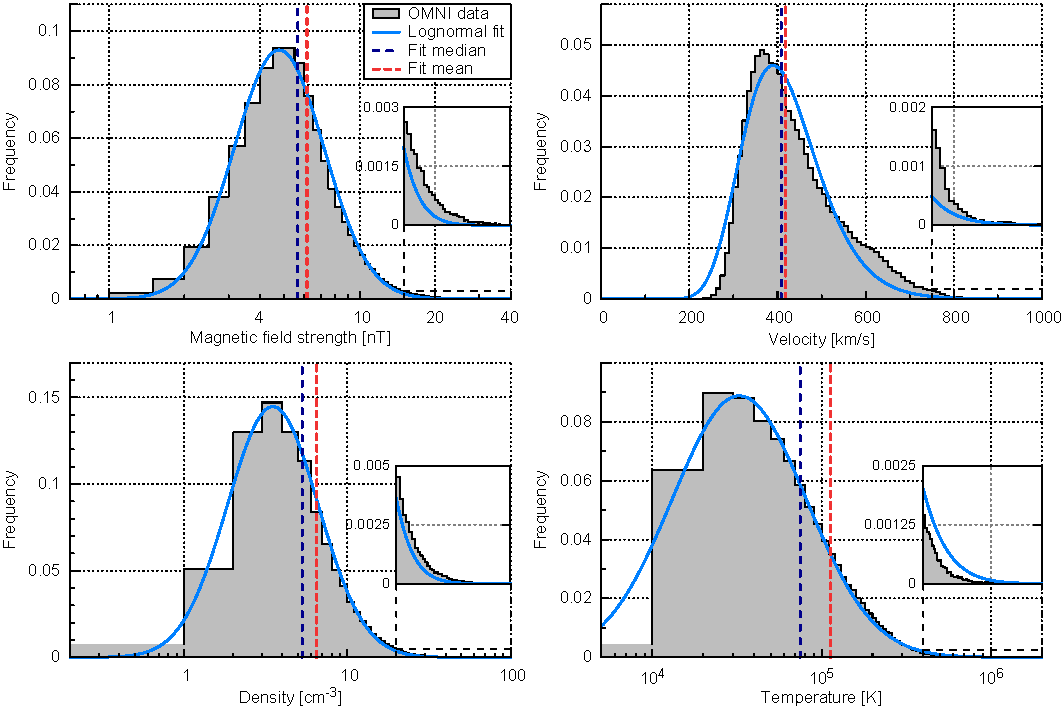
\includegraphics[width=18cm]{figures/histogram_fits_4_a_zoom_paper_pdfplot.pdf}
	\caption{Frequency distributions of the four solar wind parameters and their lognormal fits. The histograms have bins of 0.5~nT, 10~km/s, 1~cm$^{-3}$ and 10\,000~K and are based on the hourly OMNI data set. The fit's median and mean values are indicated as well. The insets only have zoomed-in frequency axes, their x-axes stay the same.}
	\label{fig:histogram_fits_4_a_zoom_paper_pdfplot}
\end{figure*}

%double lognormal fitting
%%%%%%%%%%%%%%%%%%%%%%%%%
%justification for compositional lognormal fit
To reach a better fit result for the velocity we change the fit function. We do not want to abandon the well-founded application of the lognormal function. However, it is reasonable to assume that the velocity distribution is composed of at least two branches (slow and fast). Therefore a compositional approach promises better fit results, which is why we combine two lognormal functions (\ref{eq:single_lognormal_fit_function}), bearing the disadvantage of more fit variables:
\begin{align}
	W_\text{II}(x) &= c \cdot W_1(x) + (1 -c) \cdot W_2(x)\,.	\label{eq:double_lognormal_fit_function}
\end{align}
The balancing parameter $c$ ensures that the resulting function remains normalized as it represents a probability distribution.

The fitting of $W_\text{II}(x)$ to the velocity's frequency distribution gives the values of the now five fit parameters ($c$, $x_\text{med,1}$, $x_\text{avg,1}$, $x_\text{med,2}$ and $x_\text{avg,2}$), which are also listed in Table~\ref{tab:lognormal_fit_parameters} together with the median and mean of the composed distribution, which can be derived via solving
\begin{align}
	\int W_\text{II}(x)\,\text{d}x = 0	&	&\text{and}	&	&\int x\,W_\text{II}(x)\,\text{d}x = 0
\end{align}
respectively.\\
As anticipated, this more complex fit function is more accurate in describing the velocity's frequency distribution (see Fig.~\ref{fig:histogram_fits_V_a_zoom_dbl_paper_pdfplot}).
\begin{figure}
	\resizebox{\hsize}{!}{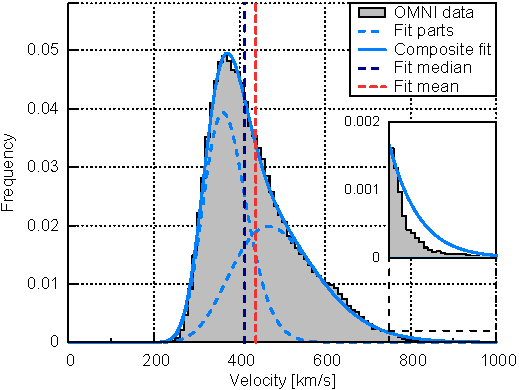
\includegraphics{figures/histogram_fits_V_a_zoom_dbl_paper_pdfplot.pdf}}
	\caption{Plot of the velocity's frequency distribution (same as in Fig.~\ref{fig:histogram_fits_4_a_zoom_paper_pdfplot}) and its compositional lognormal fit. The fit's median and mean values and its two fit parts are indicated as well. The inset only has a zoomed-in frequency axis, its x-axis stays the same.}
	\label{fig:histogram_fits_V_a_zoom_dbl_paper_pdfplot}
\end{figure}
That is why we keep using the double lognormal ansatz for the velocity frequency fits in the following sections.\\
In this static model the slow and fast part contribute almost equally ($c \approx 0.5$), which of course is only valid for this kind of long-term average. At different times in a solar cycle their contributions vary strongly.\\

%transition
For the bulk of the solar wind these static lognormal functions describe the parameters' distributions well. This is different for the extreme values (which may also stem from CMEs). The simple lognormal fit models of the magnetic field strength, the velocity and the density underestimate their frequency at the high value tails, whereas the temperature's tail is overestimated (see insets of Fig.~\ref{fig:histogram_fits_4_a_zoom_paper_pdfplot}). The velocity's compositional lognormal fit only slightly overestimates its tail (inset in Fig.~\ref{fig:histogram_fits_V_a_zoom_dbl_paper_pdfplot}).\\

Short-term variations in the solar wind cannot be predicted, but their occurrence rate can. It depends on solar activity, which changes cyclically and thus can be forecasted to a certain degree---at least within a solar cycle.\\


\section{Solar activity variations}
\label{sec:solar_activity_variations}
This section aims to relate changes in the four solar wind parameters to general solar activity. For this we examine their correlations to the yearly sunspot number and determine the lag times with the highest coefficients. Next, we fit lognormal functions to the frequency distributions like before, but implement linear relations to the yearly SSN to shift the distributions. Only for the velocity the approach is different in that its two components are kept fixed and instead their balance is modified with changing SSN.

\subsection{SSN data}
Solar activity is commonly measured via the sunspot number. We want to correlate OMNI in situ measurements with the SSN, but OMNI data are from Earth orbit, causing variations in solar latitude and distance. To dodge these variations we use yearly OMNI and SSN data.\\

The international sunspot number (\citeyear{sidc}) is retrieved from the online catalogue\footnote{\url{http://www.sidc.be/silso/}} at the World Data Center -- Sunspot Index and Long-term Solar Observations (WDC-SILSO), Solar Influences Data Analysis Center (SIDC), Royal Observatory of Belgium (ROB).\\

seasonal influence contained within yearly frequency distributions\\

SIDC and SWPC provide limited SSN forecast (a few months)\\

\subsection{SSN correlation}
Our current interest lies in the correlation of the SSN to the solar wind median value, because it defines the position of the lognormal function. The yearly OMNI parameter medians and the yearly SSN are plotted in Fig.~\ref{fig:OMNI_yearly_ssn_correlation_b_plot}.\\

solar activity = SSN $\neq$ solar cycle\\
The solar wind velocity (and its close friends N \& T) is known to depend on the state of the solar cycle (cite?), which is why it follows the SSN only indirectly (with time lag). Thus we derive the correlation coefficients for different time lags between solar wind parameters and SSN (see Fig.~\ref{fig:OMNI_yearly_ssn_correlation_b_plot}).\\
\begin{figure}
	\resizebox{\hsize}{!}{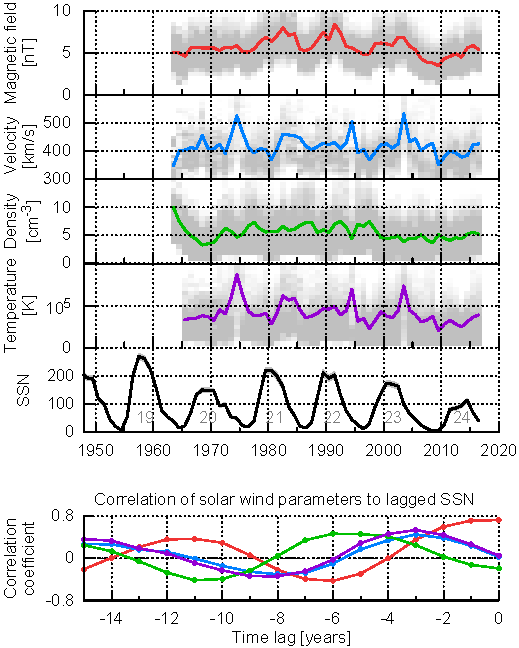
\includegraphics{figures/OMNI_yearly_ssn_correlation_b_plot.pdf}}
	\caption{Plot of the solar wind parameter yearly medians from OMNI data and the yearly SSN from the \citet{sidc} with cycle number (top). Their correlation coefficients with the yearly SSN for time lags back to -15 years (bottom).}
	\label{fig:OMNI_yearly_ssn_correlation_b_plot}
\end{figure}

The highest correlation coefficient for the magnetic field strength is 0.728. It is without lag time and the highest of all solar wind parameters, which is expected because the SSN is directly proportional to the solar surface magnetic flux (cite?).\\
Velocity and temperature have a lag time of 3~years with their maximal correlation coefficients (0.453 and 0.540). The density even 6~years (0.468).\\
% maximal correlation coefficients and their lag times:\\
% magnetic field strength: lag 0, 0.728\\
% velocity: lag -3, 0.453\\
% density: lag -6, 0.468\\
% temperature: lag -3, 0.540\\

cause: direct/indirect correlation\\
cite literature to lag time...\\

yearly SSN sw model to sw data fits -> SSN dependency (new figs)\\

\subsection{SSN fitting}
\label{sec:ssn_fitting}
To be able to shift the distributions with SSN, add fit a linear SSN dependency to the median
\begin{align}
	x_\text{med}(ssn) &= a_\text{med} \cdot ssn + b_\text{med}\,,	\label{eq:median_with_ssn}
\end{align}
using a factor to the SSN $a_\text{med}$ with a baseline $b_\text{med}$. We relate the mean with a scaling factor to the median to keep the new SSN dependency:
\begin{align}
	x_\text{avg}(ssn) &= (1 + a_\text{avg}) \cdot x_\text{med}(ssn)\,.	\label{eq:mean_with_ssn}
\end{align}
With the implementation of these relations into the lognormal function (\ref{eq:single_lognormal_fit_function}), the new dynamic fit function $W'(x,ssn)$ is then fitted to the yearly data. The three resulting fit coefficients ($a_\text{med}, b_\text{med}$ and $a_\text{avg}$) are presented in Table~\ref{tab:ssn_fit_parameters}.\\
\begin{table*}
	\caption{Resulting fit coefficients from the data fitting with SSN. For the velocity the fit parameters from the double lognormal fit and their balancing function are given. The values in brackets are the estimated standard deviation of each fit parameter.}
	\label{tab:ssn_fit_parameters}
	\centering
	\begin{tabular}{l@{} c@{}
		S[table-format = 1.3(2)e+1]
		S[table-format = 1.4(2)]
		S[table-format = 1.3(2)e+1]
		S[table-format = +1.3(2)e+1]
		c
		}
		\hline\hline
		\multicolumn{2}{l}{\multirow{2}{*}{Parameter}}	&\multicolumn{2}{c}{Median}	&\multicolumn{1}{c}{Mean}	&\multicolumn{2}{c}{Balance}\\
		\cline{3-4}\cline{6-7}
		\multicolumn{2}{l}{}	&\multicolumn{1}{c}{SSN factor $a_\text{med}$\tablefootmark{a}}	&\multicolumn{1}{c}{Baseline $b_\text{med}$\tablefootmark{a}}	&\multicolumn{1}{c}{Scaling factor $a_\text{avg}$}	&\multicolumn{1}{c}{SSN factor $c_a$}	&\multicolumn{1}{c}{Baseline $c_b$}\\
		\hline
		\multicolumn{2}{l}{Magnetic field}	&1.309(19)e-2	&4.285(17)	&8.786(78)e-2	&\multicolumn{1}{c}{--}	&--\\
%		\multicolumn{2}{l}{Velocity}	&2.514(93)e-3	&3.8521(90)	&2.392(26)e-2	&\multicolumn{1}{c}{--}	&--\\
		\multicolumn{2}{l}{Density}	&3.81(25)e-3	&4.495(26)	&3.050(27)e-1	&\multicolumn{1}{c}{--}	&--\\
		\multicolumn{2}{l}{Temperature}	&1.974(26)e-2	&5.729(19)	&6.541(28)e-1	&\multicolumn{1}{c}{--}	&--\\
		\hline
		\multirow{2}{*}{Velocity}	&\multicolumn{1}{c}{$W_1$}	&\multicolumn{1}{c}{--}	&3.633(12)	&1.008(37)e-2	&\multirow{2}{*}{\tablenum{-1.799(95)e-3}}	&\multirow{2}{*}{0.638(32)}\\
			&\multicolumn{1}{c}{$W_2$}	&\multicolumn{1}{c}{--}	&4.831(81)	&2.31(20)e-2	&	&\\
		\hline
	\end{tabular}
	\tablefoot{
		\tablefoottext{a}{Values in their respective units \si{nT}, \SI{e2}{\km\per\s}, \si{\per\cm\cubed} and \SI{e4}{\K}.}
	}
\end{table*}

In comparison with the data the fit models seem to match with the general trends (Fig.~\ref{fig:OMNI_yearly_BVdblNTSSN_fit_d_plot}).\\
\begin{figure*}
	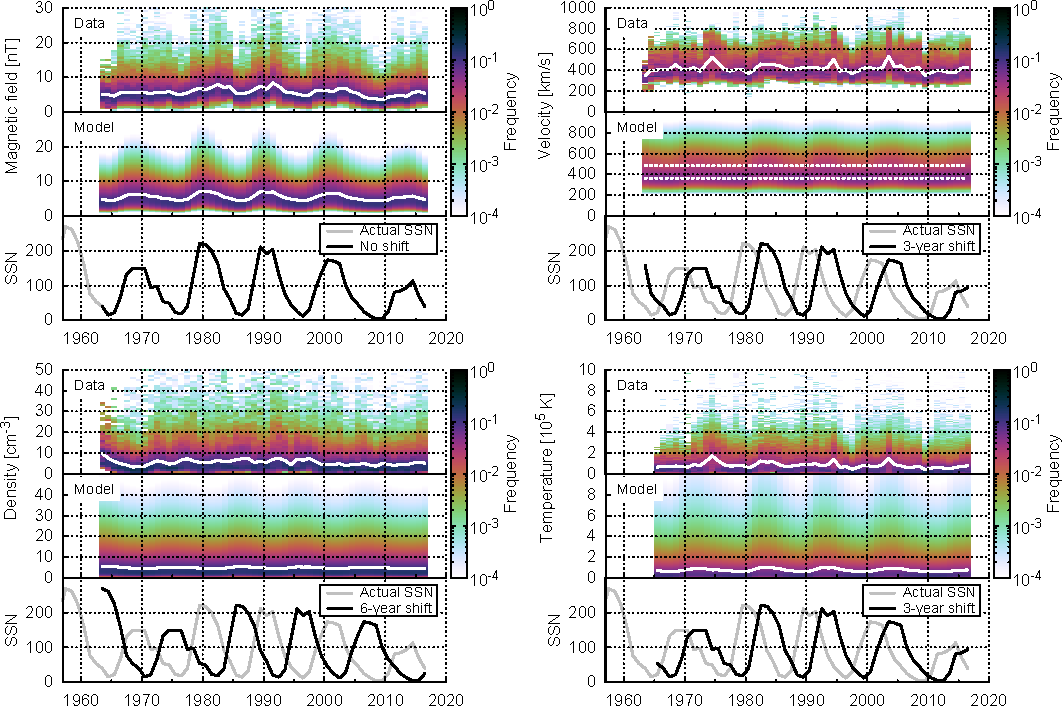
\includegraphics[width=18cm]{figures/OMNI_yearly_BVdblNTSSN_fit_d_plot.pdf}
	\caption{Solar wind parameter data frequencies, lognormal fit models with their median values (white) and the corresponding yearly SSN (grey) over the OMNI time period 1963--2016. The for the models shifted SSN is indicated by a black line. The constant medians of both velocity's lognormal parts are marked with white dots.}
	\label{fig:OMNI_yearly_BVdblNTSSN_fit_d_plot}
\end{figure*}

Again, the velocity gets a special treatment with the double lognormal distribution (\ref{eq:double_lognormal_fit_function}). It is known that slow and fast solar wind stream occurrence rates follow the solar cycle, but their magnitudes stay fairly stable (cite?). This time we keep the two velocity components' positions constant and vary instead their balance with the SSN:
\begin{align}
	c(ssn) &= c_a \cdot ssn + c_b\,.
\end{align}
The fit result (see Table~\ref{tab:ssn_fit_parameters}) is a model in which three years after solar cycle minimum (SSN of zero) the slow solar wind has a share of almost two-thirds and decreases further with increasing SSN (see Fig.~\ref{fig:Vdbl_SSN_ratio_b_plot}).\\
\begin{figure}
	\resizebox{\hsize}{!}{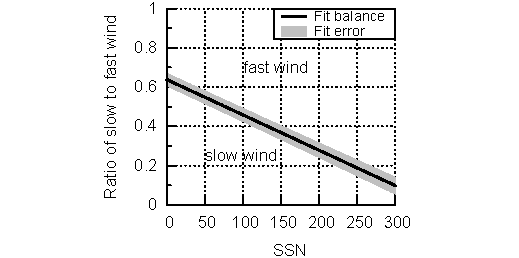
\includegraphics{figures/Vdbl_SSN_ratio_b_plot.pdf}}
	\caption{Yearly ratio between slow to fast solar wind (threshold \SI{400}{\km\per\s} over SSN (+). Fit model ratio depending on the by 3~years lagged SSN (black line). The relation results from the velocity's double lognormal fit.}
	\label{fig:Vdbl_SSN_ratio_b_plot}
\end{figure}
% 3 years after minimum (SSN of zero) the slow wind has its maximal share of 0.638(32). 3 years after maximum (SSN of 200) it has only a share of 0.278(37).\\
...compare with data\\
=> there is no specific velocity threshold between slow and fast solar wind types, the velocity ranges of both types overlap.\\

In comparison with the data the fit model roughly matches with the general trend (see Fig.~\ref{fig:OMNI_yearly_BVdblNTSSN_fit_d_plot}).\\

density modulation with SSN \citep{Schwenn1983} p.~499\\
density anticorrelation with SSN \citep{Bougeret1984} p.~406\\


%exponential fitting
%%%%%%%%%%%%%%%%%%%%
\section{Solar distance dependency}
\label{sec:solar_distance_dependency}

In this section we use Helios data to obtain exponential fit functions for the heliocentric distance dependency and evaluate the fits' extrapolation behavior in direction to the Sun. To fit the bulk solar wind distributions' distance dependency we use the frequency fitting method from Sect.~\ref{sec:frequency_distribution} on distance-binned Helios data. This results in models comprising of exponentially with distance shifted lognormal functions.

%Helios data
\subsection{Helios distance data}
\label{sec:helios_distance_data}

The Helios probes were the only spacecraft measuring in situ solar wind over large solar distance ranges in the inner heliosphere. We use the combined data from both Helios~1 and Helios~2 probes. Helios~1's (Helios~2's) highly elliptical orbit in the ecliptic covered a solar distance range of \SIrange{0.31}{0.98}{\au} (\SIrange{0.29}{0.98}{\au}). Launched during solar cycle minimum, the data of both probes cover the rise to the maximum of cycle 21 ($\sim$6.5~years at varying distances).

Helios~1's (Helios~2's) merged hourly data set from the magnetometer and plasma instruments \citep{Rosenbauer1977} includes $\sim$12.5~orbits ($\sim$8~orbits) in the time range \mbox{1974-12-10} to \mbox{1981-06-14} (\mbox{1976-01-01} to \mbox{1980-03-04}).
%Helios plasma instrument (E1); Helios magnetometer instrument (E2)
% Helios data ranges:\\
% - time range Helios~1 [1974-12-10--1981-06-14] (12.5~orbits), Helios~2 [1976-01-01--1980-03-04] (8~orbits)\\
% - solar distance range Helios~1 0.31--0.98~au, Helios~2 0.29--0.98~au\\
%data sources
The Helios data was retrieved from the Coordinated~Data~Analysis~Web (CDAWeb) interface at NASA's GSFC/SPDF\footnote{\url{http://spdf.gsfc.nasa.gov/}}.

The Helios~1 (Helios~2) magnetometer data coverage is about 43~\% (54~\%) and amounts to 2.8~years (2.3~years) in total. The plasma data coverage is 76~\% (92~\%) and amounts to 5.0~years (3.9~years) in total.
% temporal coverage of merged data\\
% Helios 1: 1974-12-10--1981-06-14; 6y6m15d = 2388~d = 6.538~y\\
% Mag data coverage: 42.6~\%; 2.785~years\\
% Plasma data coverage: 76.4~\%; 4.995~years\\
% Helios 2: 1976-01-01--1980-03-04; 4y3m4d = 1557~d = 4.263~y\\
% Mag data coverage: 54.4~\%; 2.319~years (83~\% of H1)\\
% Plasma data coverage: 91.8~\%; 3.913~years (78~\% of H1)\\
Thus, the Helios data cover only fractions of a solar cycle and cannot be used for deriving representative time-independent solar wind multi-cycle conditions like the OMNI data can.

%Helios data biased towards solar minimum
Using this data, we also have to keep in mind that its time coverage is unequally distributed over the solar cycle. Dividing the data by the transition from cycle minimum to maximum (mid 1977) and considering the data gap distributions, the Helios data covers about \SI{68}{\percent} during cycle minimum whereas during maximum only \SI{38}{\percent}.\\

% data gaps -> uneven coverage -> solar cycle minimum dominates; ratio of max vs min cycle data coverage; for OMNI data negligible\\
% 13~months smoothed sunspot number \citep{sidc}: divide June~1977 (include figure)\\
% put link on sidc webpage: http://sidc.be/sunspot-data/SIDCpub.php
% begin: 1974-12 36.1\\
% minimum: May/June 1976 18.3/17.9 (cite?)\\
% divide 30~June~1977 37.7 from SIDC data (nearly same SSN as at Helios~1 beginning)\\
% cycle 21 maximum: Dec 1979 232.9 (cite?)\\
% end: 1981-06 200.9\\
% 
% data gap hours and percentages:\\
% % H1 minimum 22416 h\\
% % H1 maximum 34681 h\\
% % H2 minimum 13128 h\\
% % H2 maximum 23472 h\\
% % sum 93697 h\\
% solar minimum: 35\,544~h, 37.94~\%\\
% solar maximum: 58\,153~h, 62.06~\%\\

% 1974 11 1974.874   39.3   4.2    30  
% 1974 12 1974.958   36.1   4.0    31  
% 1975 01 1975.042   33.0   3.9    31  
% 1975 02 1975.123   31.8   3.8    28  
% 1975 03 1975.204   30.6   3.7    31  
% 1975 04 1975.288   26.8   3.5    30  
% 1975 05 1975.371   24.2   3.3    31  
% 1975 06 1975.455   23.2   3.3    30  
% 1975 07 1975.538   21.8   3.2    31  
% 1975 08 1975.623   20.7   3.1    31  
% 1975 09 1975.707   20.9   3.1    30  
% 1975 10 1975.790   22.3   3.2    31  
% 1975 11 1975.874   23.3   3.3    30  
% 1975 12 1975.958   23.6   3.3    31  
% 1976 01 1976.042   22.1   3.2    31  
% 1976 02 1976.124   19.2   3.0    29  
% 1976 03 1976.206   17.8   2.9    31  
% 1976 04 1976.290   18.4   2.9    30  
% 1976 05 1976.373   18.3   2.9    31  
% 1976 06 1976.456   17.9   2.9    30  
% 1976 07 1976.540   18.8   2.9    31  
% 1976 08 1976.624   20.5   3.1    31  
% 1976 09 1976.708   20.8   3.1    30  
% 1976 10 1976.791   19.7   3.0    31  
% 1976 11 1976.874   19.7   3.0    30  
% 1976 12 1976.958   21.6   3.2    31  
% 1977 01 1977.042   24.3   3.3    31  
% 1977 02 1977.123   26.3   3.5    28  
% 1977 03 1977.204   28.8   3.6    31  
% 1977 04 1977.288   31.9   3.8    30  
% 1977 05 1977.371   34.7   4.0    31  
% 1977 06 1977.455   37.7   4.1    30  
% 1977 07 1977.538   41.4   4.3    31  
% 1977 08 1977.623   47.6   4.6    31  
% 1977 09 1977.707   55.8   5.0    30  
% 1977 10 1977.790   64.8   5.4    31  
% 1977 11 1977.874   73.7   5.7    30  
% 1977 12 1977.958   80.7   6.0    31  
% 1978 01 1978.042   86.9   6.2    31  
% 1978 02 1978.123   91.5   6.4    28  
% 1978 03 1978.204   98.7   6.6    31  
% 1978 04 1978.288  109.0   7.0    30  
% 1978 05 1978.371  117.8   7.2    31  
% 1978 06 1978.455  126.6   7.5    30  
% 1978 07 1978.538  138.0   7.8    31  
% 1978 08 1978.623  147.3   8.1    31  
% 1978 09 1978.707  153.6   8.3    30  
% 1978 10 1978.790  157.3   8.4    31  
% 1978 11 1978.874  160.4   8.5    30  
% 1978 12 1978.958  166.7   8.6    31  
% 1979 01 1979.042  175.2   8.8    31  
% 1979 02 1979.123  185.4   9.1    28  
% 1979 03 1979.204  193.3   9.3    31  
% 1979 04 1979.288  199.9   9.4    30  
% 1979 05 1979.371  208.5   9.6    31  
% 1979 06 1979.455  216.7   9.8    30  
% 1979 07 1979.538  219.5   9.9    31  
% 1979 08 1979.623  220.1   9.9    31  
% 1979 09 1979.707  220.4   9.9    30  
% 1979 10 1979.790  223.4  10.0    31  
% 1979 11 1979.874  229.8  10.1    30  
% 1979 12 1979.958  232.9  10.2    31  
% 1980 01 1980.042  232.0  10.2    31  
% 1980 02 1980.124  230.2  10.2    29  
% 1980 03 1980.206  227.9  10.1    31  
% 1980 04 1980.290  224.6  10.0    30  
% 1980 05 1980.373  221.3  10.0    31  
% 1980 06 1980.456  219.1   9.9    30  
% 1980 07 1980.540  216.1   9.9    31  
% 1980 08 1980.624  212.0  10.0    31  
% 1980 09 1980.708  211.5  10.2    30  
% 1980 10 1980.791  211.9  10.5    31  
% 1980 11 1980.874  209.1  10.9    30  
% 1980 12 1980.958  202.8  11.0    31  
% 1981 01 1981.042  199.6  11.1   271  
% 1981 02 1981.123  202.2  11.5   229  
% 1981 03 1981.204  205.4  12.1   244  
% 1981 04 1981.288  205.7  12.6   254  
% 1981 05 1981.371  204.1  12.8   268  
% 1981 06 1981.455  200.9  13.1   227  
% 1981 07 1981.538  198.5  13.1   268  

For calculating the median and mean values at different solar distances the data is binned into \SI{0.01}{\au} bins, which is also the native precision in this data set.\\

\subsection{Exponential fitting}
%why exponential function?
An exponential distance behavior is expected from all four parameters (cites?). Therefore we use the exponential function
\begin{align}
	x(r) = a\,r^b	\label{eq:exponential_function}
\end{align}
with the solar distance $r$ for the regression fit of the median and mean. The fits are weighted by data counts per bin.
%fit result table and figure
With $r$ in astronomical units we get the fit coefficients ($a_\text{med}$, $a_\text{avg}$, $b_\text{med}$ and $b_\text{avg}$) as given in Table~\ref{tab:mean_median_fit_parameter}.\\
\begin{table*}
	\caption{These are the fit coefficients for the median and mean solar distance dependencies of the four parameters from the combined Helios data set. The errors in brackets are the estimated standard deviations of each fit parameter. The crossing distance is the point where the fitted median and mean intersect.}
	\label{tab:mean_median_fit_parameter}
	\centering
	\begin{tabular}{l
	S[table-format = 1.3(2)]
	S[table-format = +1.3(2)]
	@{}c
	S[table-format = 1.3(2)]
	S[table-format = +1.3(2)]
	S[table-format = 1.1(2)e1]}
		\hline\hline
		\multirow{2}{*}{Parameter}	&\multicolumn{2}{c}{Median}	&	&\multicolumn{2}{c}{Mean}	&\multicolumn{1}{c}{Crossing distance}\\
		\cline{2-3}	\cline{5-6}
			&\multicolumn{1}{c}{$a_\text{med}$\tablefootmark{a}}	&\multicolumn{1}{c}{$b_\text{med}$}	&	&\multicolumn{1}{c}{$a_\text{avg}$\tablefootmark{a}}	&\multicolumn{1}{c}{$b_\text{avg}$}	&\multicolumn{1}{c}{[\si{\au}]}\\
		\hline
		Magnetic field	&5.377(92)	&-1.655(17)	&	&6.05(10)	&-1.546(18)	&0.339(11)\\
		Velocity	&4.107(28)	&0.058(13)	&	&4.356(24)	&0.049(10)	&0.7(83)e3\\
		Density		&5.61(27)	&-2.093(46)	&	&7.57(30)	&-2.010(38)	&0.027(73)\\
		Temperature	&7.14(23)	&-0.913(39)	&	&9.67(21)	&-0.792(28)	&0.082(85)\\
		\hline
	\end{tabular}
	\tablefoot{
		\tablefoottext{a}{Values in their respective units \si{nT}, \SI{e2}{\km\per\s}, \si{\per\cm\cubed} and \SI{e4}{\K}.}
	}
\end{table*}

%crossing distances
The next step is to fit the bulk of the solar wind parameters with lognormal functions. At all considered solar distances the mean of the three plasma parameters is larger than their median (Fig.~\ref{fig:radial_fit_4_thesis_light_skip_pdfcairo_plot}).
\begin{figure*}
	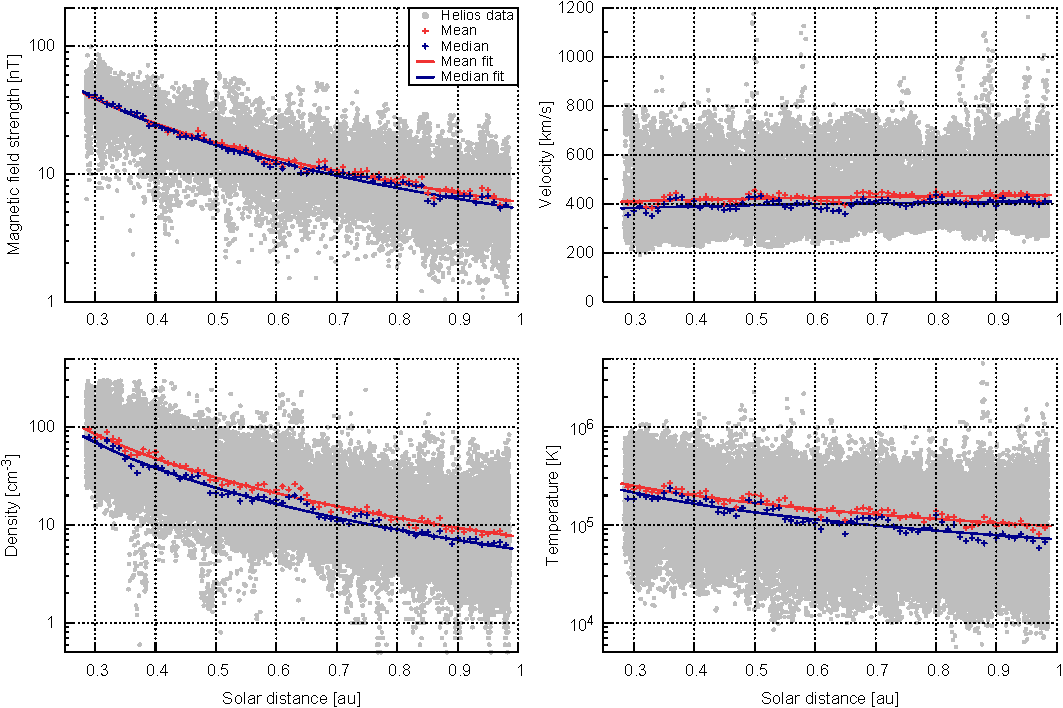
\includegraphics[width=18cm]{figures/radial_fit_4_thesis_light_skip_pdfcairo_plot.pdf}
	\caption{Helios hourly data plots of the four solar wind parameters over solar distance. The mean and median per \SI{0.01}{\au} data bin and their fit curves are plotted as well. The Helios data has a native distance resolution of \SI{0.01}{\au}. To make the abundance visible in these plots, we added a random distance value of up to \SI{+-0.005}{\au}.}
	\label{fig:radial_fit_4_thesis_light_skip_pdfcairo_plot}
\end{figure*}
However, the magnetic field strength's mean crosses the median at \SI{0.339}{\au} (Table~\ref{tab:mean_median_fit_parameter}) and is lower at smaller distances. At the crossing point and below the magnetic field strength can therefore not be described anymore with a lognormal function. For an extrapolation to the SPP perihelion the same happens for the temperature at \SI{0.082}{\au}.

The large velocity's crossing distance and its large error indicate that the median's and mean's distance behavior can be kept identical and so the frequency's shape distance independent.

Those crossings limit the possible extrapolation distances with lognormal functions. To circumvent these limitations for all four solar wind parameters we set the exponents $b_\text{med}$ and $b_\text{avg}$ to be identical, avoiding crossing of median and mean. Then the distribution's width is constant and scales only exponentially with solar distance. Applying this approximation, we have to accept larger model errors, especially for the magnetic field strength. It also limits the extrapolation accuracy.

\subsection{Exponential lognormal fitting}
To retrieve the frequency distributions for every \SI{0.01}{\au} solar distance bin, we choose the same solar wind parameter binning as with the OMNI data (Sect.~\ref{sec:omni_frequency_data}).\\
% Helios histogram bin sizes for mean of frequency distribution (at specific solar distance):\\
% $B$: bin size 0.5~nT, min 337, mean precision: 0.000545\\
% $v$: bin size 1~cm$^{-3}$, min 497, mean precision: 0.00449\\
% $n$: bin size 10~km/s, min 497, mean precision:  0.00449\\
% $T$: bin size 10\,000~K, min 497, mean precision: 4.49--44.49\\

As mentioned before, we set the exponents of median and average to be identical. Implementing the exponential distance dependency~(\ref{eq:exponential_function}) into the lognormal function (\ref{eq:single_lognormal_fit_function}), we get three fit parameters ($a_\text{med}$, $a_\text{avg}$ and the common exponent $b$).

Naturally, we use the double lognormal function~(\ref{eq:double_lognormal_fit_function}) for the velocity distribution fit, resulting in $W''_\text{II}(x,r)$. The additional fit parameters are the balancing parameter $c$ and from the second lognormal part $a_\text{med,2}$ and $a_\text{avg,2}$. The resulting fit coefficients for the four solar wind parameters are presented in Table~\ref{tab:extrapolation_model_fit_parameters}.
\begin{table*}
	\caption{These are the resulting fit coefficients with the single lognormal exponential function, respectively double lognormal for the velocity. The errors in brackets are the estimated standard deviations of each fit parameter.}
	\label{tab:extrapolation_model_fit_parameters}
	\centering
	\sisetup{table-figures-integer=1, table-figures-decimal=3, table-figures-exponent=0}
	\begin{tabular}{l c
	S[table-format = 1.3(2), table-space-text-post = a, table-align-text-post = false]
	S[table-format = 1.3(2), table-space-text-post = a, table-align-text-post = false]
	S[table-format = +1.4(2)]
	S[table-format = 1.3(2)]}
		\hline\hline
		\multicolumn{2}{l}{Parameter}	&\multicolumn{1}{c}{$a_\text{med}$\tablefootmark{a}}	&\multicolumn{1}{c}{$a_\text{avg}$\tablefootmark{a}}	&\multicolumn{1}{c}{$b$}	&$c$\\
		\hline
		\multicolumn{2}{l}{Magnetic field}	&5.358(25)	&5.705(28)	&-1.662(11)	&\multicolumn{1}{c}{--}\\
		\multicolumn{2}{l}{Density}	&5.424(33)	&6.845(47)	&-2.114(20)	&\multicolumn{1}{c}{--}\\
		\multicolumn{2}{l}{Temperature}	&6.357(64)	&10.72(14)	&-1.100(20)	&\multicolumn{1}{c}{--}\\
		\hline
		\multirow{1}{*}{Velocity}	&$W''_1$	&3.707(13)	&3.748(16)	&\multirow{2}{*}{0.0990(51)}	&\multirow{2}{*}{0.557(45)}\\
			&$W''_2$	&5.26(13)	&5.42(11)	&	&\\
		\cline{2-6}
		\multicolumn{2}{r}{$W''_\text{II}$}	&4.35(13)\tablefootmark{b}	&4.77(11)\tablefootmark{b}	&\multicolumn{1}{c}{--}	&\multicolumn{1}{c}{--}\\
		\hline
	\end{tabular}
	\tablefoot{
		\tablefoottext{a}{Values in their respective units \si{nT}, \SI{e2}{\km\per\s}, \si{\per\cm\cubed} and \SI{e4}{\K}.}
		\tablefoottext{b}{Velocity median and mean \SI{1}{\au} values for the resulting function. Error estimates derived from the individual fit part errors.}
	}
\end{table*}

With $c = 0.557$ the velocity balancing parameter is of an expected value similar to that obtained from the Helios time period (the mean SSN during the Helios period was 59, this corresponds to a $c(59) = 0.53$, see Fig.~\ref{fig:Vdbl_SSN_ratio_b_plot}).\\

The fit models seem to resemble the data quite well (Fig.~\ref{fig:mixed_fit_fixed_4_paper_e_plot}). The magnetic field strength frequency is more focused (around \SI{40}{nT}) at the lower distance boundary than the model's is. This is expected because of our fixed distance independent shape approximation.\\
\begin{figure*}
	\includegraphics[width=18cm]{figures/mixed_fit_fixed_4_paper_e_plot.pdf}
	\caption{Solar wind parameter's frequency distributions over solar distance. Plotted are the binned Helios data and the exponential lognormal fit model (double lognormal for the velocity) with their median values (white).}
	\label{fig:mixed_fit_fixed_4_paper_e_plot}
\end{figure*}

model errors, maximum errors\\
The extreme values of the velocity and temperature seem to be too high (adjust color scale...)\\
L-> high value plots... (refer to histogram zoom in Fig.~\ref{fig:histogram_fits_4_a_zoom_paper_pdfplot})\\

This model represents the Helios time frame around the rise of solar cycle~21.\\

study time/cycle variations\\
indications for that: fig. + theory + studies/papers...\\
assuming the distance scaling laws are time independent, which we deduced...? which is an approximation.\\


\section{General solar wind model}
\label{sec:general_solar_wind_model}

Finally, we combine the obtained solar activity and distance dependencies for shifting the frequency distributions. The result is an empirical solar wind model for the inner heliosphere.\\

%are the exponents time-independent?
Under the assumption that the exponential falloff laws do not change with time/solar activity (as shown above...), they can be used in general.\\

We combine the fit coefficients of the median relation for solar activity dependence (\ref{eq:median_with_ssn}) with the ones from the exponential distance dependence (\ref{eq:exponential_function})
\begin{align}
	x_\text{med}(ssn,r) &= (a_\text{med} \cdot ssn + b_\text{med}) \cdot r^b
\end{align}

to get the combined model function $W''(x,ssn,r)$. And for the velocity $W_{II}''(x,ssn,r)$ with the double lognormal function.\\

%model errors
give model errors sizes/uncertainties (sigmas); $W''_\text{err}(x,ssn,r)$, $x_\text{med\_err}(ssn,r)$


\section{Model extrapolation to SPP orbital time and position}
To estimate the solar wind environment at SPP's planned orbital positions during its mission time, SSN predictions and extrapolations to the SPP perihelion region are included into the general solar wind model.\\

%SPP orbit
SPP orbit description, Venus flybys, within ecliptic, \citep{Fox2015}, (see Fig.~\ref{fig:SPP_orbit_predicted_SSN_overview_b_plot})\\

%SSN prediction
choosing SSN prediction sources as input:\\
SIDC prediction---12-month forecast (Kalman fiter combined method)\\
The SWPC prediction (until end of current cycle/end of 2019) follows a consensus of the Solar~Cycle~24 Prediction~Panel.\\
For the prediction of the next solar cycle we simply assume a course similar to the last and thus we simply shift the last cycle by 11~years. Additionally we consider the two alternatives of half and twice the amplitude.\\
SIDC + SWPC + previous cycle~24 (see Fig.~\ref{fig:SPP_orbit_predicted_SSN_overview_b_plot})\\
\begin{figure}
	\resizebox{\hsize}{!}{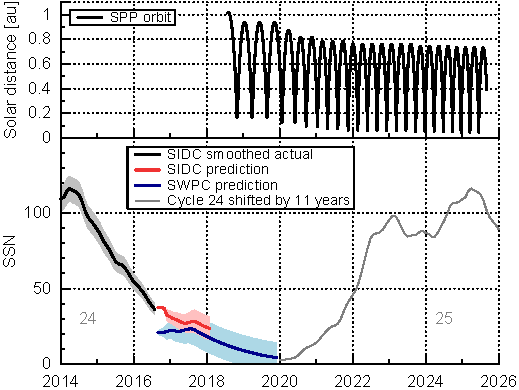
\includegraphics{figures/SPP_orbit_predicted_SSN_overview_b_plot.pdf}}
	\caption{SPP's solar distance during its mission time (top). Consecutive Venus flybys bring its perihelia nearer to the Sun. Actual and predicted SSN (bottom), i.e. SIDC 13-month smoothed monthly actual SSN, SIDC prediction, SWPC prediction and simply shifted SSN from previous cycle~24, together with two alternative trends of half and twice the amplitude.}
	\label{fig:SPP_orbit_predicted_SSN_overview_b_plot}
\end{figure}

Implementing the orbital distance data and predicted SSN for the mission time we get SPP's estimated solar wind environment.\\
A zoom into the first and the nearest perihelia shows... (Fig.~\ref{fig:SPP_perihelia_prediction_plot}).\\
\begin{figure}
	\resizebox{\hsize}{!}{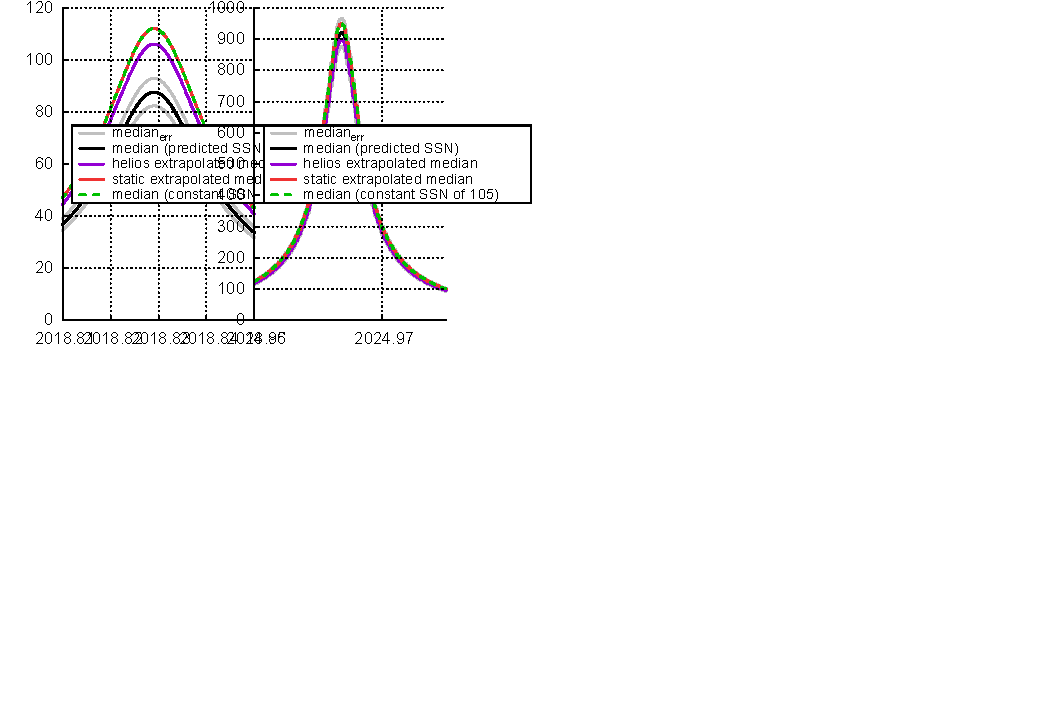
\includegraphics{figures/SPP_perihelia_prediction_plot.pdf}}
	\caption{Estimated B-field median during the first and nearest perihelia in 2018 and 2024.}
	\label{fig:SPP_perihelia_prediction_plot}
\end{figure}

\subsection{Near-Sun extrapolation behavior/effects}
The extrapolation distance is only about one third of the model range, but as the parameters follow exponential change, one has to look at the logarithmic distance which is indeed one and a half times the model range.\\

extrapolation errors...\\

velocity:\\
%critical surfaces
Alfvénic critical surface i.e. source surface (see Fox before 2.1)\\
in direction to the Sun is at $\sim$2.5~Rs the source surface (Schatten1969)\\
sonic and Alfvénic critical point positions (see \citet{Sittler1999})\\
sonic point and slow solar wind origin \citep{Sheeley1997}\\
approaching these regions, acceleration plays a role\\

The near-Sun (SPP perihelion) solar wind velocity is expected to be slower than our model estimates, because the position of the source (Alfvénic critical) surface is predicted to lie between 15--30~Rs (Schatten1969, Sittler1999, Exarhos2000, Katsikas2010, Goelzer2014; choose references...), up to which the solar wind is believed to be accelerated.\\

density:\\
\citet{Leblanc1998} -> electron density model derived from type~III radio burst observations\\
The density distance dependency scales with $r^{-2}$, but steepens below 10~Rs with $r^{-6}$ \citep{Leblanc1998}.\\

magnetic field and temperature:\\
crossing distance effect\\

Comparison with existing near-Sun models (renew extrapolation figure to 1-column):\\

\citet{Wang2000}, sources of slow solar wind + IMF regulation mechanism + blobs; compare with our slow V lognormal part\\

% comparison with other Helios studies (Schwenn, Bougeret)
\citet{Schwenn1983,Schwenn1990}, who derived the distance dependencies for both Helios spacecraft separately ($v_\text{H1}(r) \propto r^{0.083}$ and $v_\text{H2}(r) \propto r^{0.036}$), average or median? fits well...\\
Helios results, radial gradients see \citet{Schwenn1990} p.~155\\

The electron density distance function, which \citet{Bougeret1984} derived from Helios data and normed to the 1976 1~au density ($n(r) = 6.14\,r^{-2.10(4)}\,\text{cm}^{-3}$) also fits well...\\

\citet{Sheeley1997} -> LASCO coronagraph observed speed profile of coronal features tracing the slow solar wind, 2--30~Rs\\
- parabolic eq.~(2) and exponential eq.~(3)\\
- sonic point 5--6~Rs\\
- slow solar wind origin 3--4~Rs\\

The model of \citet{Sittler1999} is based on Skylab coronagraph and Ulysses data. it is a 2d semiempirical MHD model (time static)\\
L-> compare with their radial density function eq. (18a); B-field function eq. (19a+b); V(r) eq. (24); T(r)...\\

\subsection{Model requirements and limits}

model requirements:\\
- modeling the frequency distribution with sufficient accuracy -> error size (changing distribution shape with distance)\\
- modeling the distance dependency with sufficient accuracy -> error size (different scaling law at smaller distances?)\\
- possibility to extrapolate model down to 0.0459~au\\

%model limits
model limits (spherical coordinates):\\
- heliocentric distance range 0.29--0.98~au\\
- rotational symmetry\\
- confined to ecliptic +-7.2 degrees\\
model constrictions:\\
- solar distance dependency function\\
- frequency distribution functions\\
- neglected influence from heliolatitude variation\\


\subsection{Model validity and error sources}
\label{sec:model_validity_and_errors}

validity and estimation of error size outside of valid model range...\\
derive heliocentric distance depending error...\\

list simplifications/approximations...\\

error estimation for general model and extreme value tendencies\\

error sources:\\
- extrapolation\\
- lognormal model\\
- SSN variance\\

all estimates outside these boundaries are extrapolations with large uncertainties.\\

discuss high value zoom figures\\

The use of hourly data instead of higher resolution data (less than 1~min) has no significant influence on the bulk results. The minutely OMNI data frequency distributions are almost congruent and differ only slightly at their extreme ends.\\
The many hourly Helios data points which contain only a few measurements, contribute with a larger scatter to the frequency distributions \citep[p.~491]{Schwenn1983}.\\

The solar wind parameters vary with solar distance as well as with latitudinal separation from the heliospheric current sheet (HCS).\\
The OMNI data is time-shifted to the nose of the Earth's bow shock. This leads to yearly solar distance variations of \SI{>2}{\percent} (cite?) as the Earth orbits the Sun. Furthermore, its orbit within the ecliptic leads to a yearly variation of \SI{+-7.2}{\degree} in heliospheric latitude.\\
The HCS's position in latitude is highly variable around the solar equator \citep[p.~127~ff.?]{Schwenn1990}.\\

Error estimation over the year (seasonal/monthly) -> we expect variations to be less than 5~\%\\

OMNI data is not corrected for solar distace. only available for 1-/5-min data\\

%[limited parameter ranges... (minV: 171~km/s; Schwenn1983)]\\


\section{Results and discussion}

list of results:\\
- empirical solar wind model for inner heliosphere within ecliptic\\
- low velocity at 0.0459~au\\
- slow/fast ratio SSN dependency\\
- application validity of lognormal distributions\\
--> B inversion of frequency distribution\\
---> magnetic field distribution's with distance increasing high value tail -> source are compression regions (why with density no increase?); look into Parker1958's B-field formula...\\
varying shape with distance is indicator for internal physical processes (mixing/turbulence...)\\

%solar wind -> structures\\
\citet{Balogh1999} p.~162~ff (origin and formation of CIRs in inner heliosphere with Helios data; latitude V dependence)\\
Balogh2009 (HMF review + inner heliosheath)\\
Patsourakos2016 (near-Sun B-field of CMEs)\\
Aschwanden2004, p.~29\\

Parker1963\\
%https://babel.hathitrust.org/cgi/pt?id=uc1.b4264142;view=1up;seq=12

individual velocity part discussion -> there is no specific velocity threshold between slow and fast solar wind types, the velocity ranges of both types overlap.\\
\citet{Sanchez-Diaz2016} (very slow solar wind)\\
Not only the slowest wind but also the fastest wind is expected to converge to the average speed (Sanchez-Diaz2016 p.~2835, using MHD-model -> very slow solar wind is continuation of slow wind) (because of interaction).\\

The ratio of both varies with solar activity, e.g. 3~years after maximum, polar coronal holes are observed to often have equatorial extensions (cite?). see and use \citet{Bougeret1984} p.~498...\\

larger influx from higher latitudes (see figure b))\\

In most studies the density distance dependence is assumed to scale with $r^{-2}$ (cites), assuming a constant velocity.\\


\section{Conclusions}

Further investigations should be done into structure extrapolations, outward extension of model to Mars...\\

Further questions:\\
nearer to the Sun (at and below the source surface) the solar wind expansion in the ecliptic should be less spherical but more circular due to the influx from higher latitudes. => density exponent > -2\\
see Li2011 Fig.~1\\
% n	v
% -2.05	0.05
% -2	0
% -1.8	-0.2
% -1.5	-0.5


